\section*{Introduction}
Constructing a compiler is split into four categories; lexer, parser, semantic analyser and code generator, as shown in figure \ref{fig:Compilerconstruction}.
The user inputs some code, to the compiler that he would like to have compiled, which is first met by the lexer. The lexer's job is to make a token for each of the characters that is provided in the code. If a character is not recognized, this stage will fail. \\

\noindent{The parser asks the lexer for a token, which is then handled by the parser. This is being repeated until there are no tokens left. The parser's main function is to check the syntax of the source code, to check whether it contains any invalid sign of formatting. The parser is doing this by creating a parse tree, which it uses to check that all tokens are given in the right order. If the parser is able to create more than one AST (Abstract Syntax tree), the code could behave differently each time it is compiled. There are also a number of ways for a parser to build an AST, which was discussed in section \ref{Parserstrategy}. If the parser fails to build an AST, this stage will fail.} \\

\noindent{The AST is then given to the semantic analyser, which visits each node. The semantic analyser applies code from the developer to each node, in order to check if the semantic in the usercode is valid, and if not throw an exception. The semantic analyser also builds a symbol table, in order to keep track of variables.}

\noindent {The last phase of the compiler is the code generator. The code generator's main function is to translate the source code into the target code.}


\begin{figure}[! h]
\centering
	 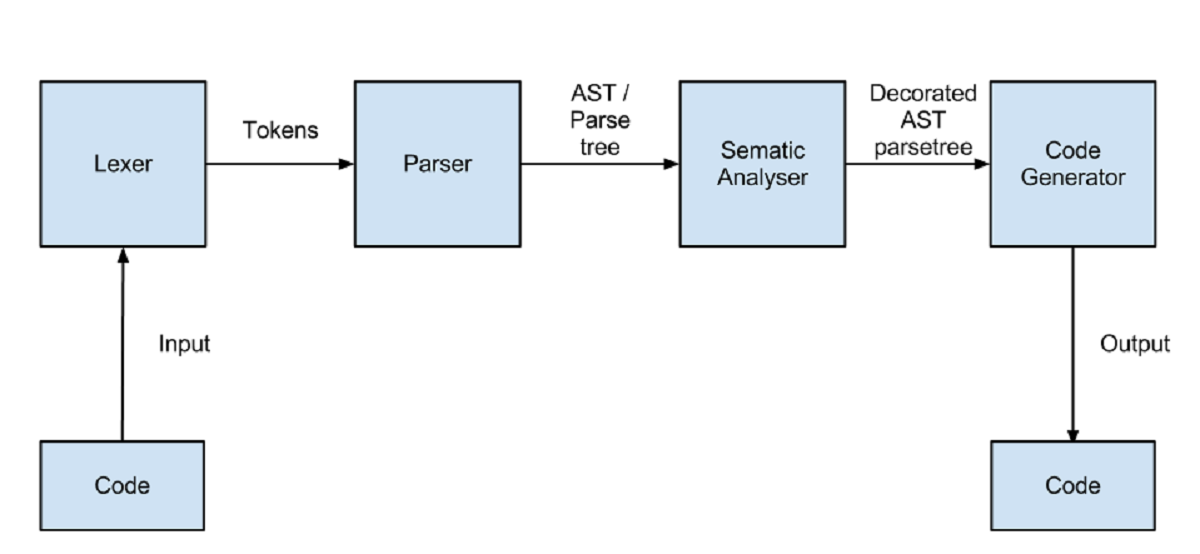
\includegraphics[width=350px]{images/Compilerconstruction1.png}
		 \caption{Compiler construction}
	\label{fig:Compilerconstruction}
\end{figure}